% Options for packages loaded elsewhere
\PassOptionsToPackage{unicode}{hyperref}
\PassOptionsToPackage{hyphens}{url}
%
\documentclass[
  a4paper,
]{article}
\usepackage{amsmath,amssymb}
\usepackage{setspace}
\usepackage{iftex}
\ifPDFTeX
  \usepackage[T1]{fontenc}
  \usepackage[utf8]{inputenc}
  \usepackage{textcomp} % provide euro and other symbols
\else % if luatex or xetex
  \usepackage{unicode-math} % this also loads fontspec
  \defaultfontfeatures{Scale=MatchLowercase}
  \defaultfontfeatures[\rmfamily]{Ligatures=TeX,Scale=1}
\fi
\usepackage{lmodern}
\ifPDFTeX\else
  % xetex/luatex font selection
\fi
% Use upquote if available, for straight quotes in verbatim environments
\IfFileExists{upquote.sty}{\usepackage{upquote}}{}
\IfFileExists{microtype.sty}{% use microtype if available
  \usepackage[]{microtype}
  \UseMicrotypeSet[protrusion]{basicmath} % disable protrusion for tt fonts
}{}
\makeatletter
\@ifundefined{KOMAClassName}{% if non-KOMA class
  \IfFileExists{parskip.sty}{%
    \usepackage{parskip}
  }{% else
    \setlength{\parindent}{0pt}
    \setlength{\parskip}{6pt plus 2pt minus 1pt}}
}{% if KOMA class
  \KOMAoptions{parskip=half}}
\makeatother
\usepackage{xcolor}
\usepackage[margin=1in]{geometry}
\usepackage{color}
\usepackage{fancyvrb}
\newcommand{\VerbBar}{|}
\newcommand{\VERB}{\Verb[commandchars=\\\{\}]}
\DefineVerbatimEnvironment{Highlighting}{Verbatim}{commandchars=\\\{\}}
% Add ',fontsize=\small' for more characters per line
\usepackage{framed}
\definecolor{shadecolor}{RGB}{248,248,248}
\newenvironment{Shaded}{\begin{snugshade}}{\end{snugshade}}
\newcommand{\AlertTok}[1]{\textcolor[rgb]{0.94,0.16,0.16}{#1}}
\newcommand{\AnnotationTok}[1]{\textcolor[rgb]{0.56,0.35,0.01}{\textbf{\textit{#1}}}}
\newcommand{\AttributeTok}[1]{\textcolor[rgb]{0.13,0.29,0.53}{#1}}
\newcommand{\BaseNTok}[1]{\textcolor[rgb]{0.00,0.00,0.81}{#1}}
\newcommand{\BuiltInTok}[1]{#1}
\newcommand{\CharTok}[1]{\textcolor[rgb]{0.31,0.60,0.02}{#1}}
\newcommand{\CommentTok}[1]{\textcolor[rgb]{0.56,0.35,0.01}{\textit{#1}}}
\newcommand{\CommentVarTok}[1]{\textcolor[rgb]{0.56,0.35,0.01}{\textbf{\textit{#1}}}}
\newcommand{\ConstantTok}[1]{\textcolor[rgb]{0.56,0.35,0.01}{#1}}
\newcommand{\ControlFlowTok}[1]{\textcolor[rgb]{0.13,0.29,0.53}{\textbf{#1}}}
\newcommand{\DataTypeTok}[1]{\textcolor[rgb]{0.13,0.29,0.53}{#1}}
\newcommand{\DecValTok}[1]{\textcolor[rgb]{0.00,0.00,0.81}{#1}}
\newcommand{\DocumentationTok}[1]{\textcolor[rgb]{0.56,0.35,0.01}{\textbf{\textit{#1}}}}
\newcommand{\ErrorTok}[1]{\textcolor[rgb]{0.64,0.00,0.00}{\textbf{#1}}}
\newcommand{\ExtensionTok}[1]{#1}
\newcommand{\FloatTok}[1]{\textcolor[rgb]{0.00,0.00,0.81}{#1}}
\newcommand{\FunctionTok}[1]{\textcolor[rgb]{0.13,0.29,0.53}{\textbf{#1}}}
\newcommand{\ImportTok}[1]{#1}
\newcommand{\InformationTok}[1]{\textcolor[rgb]{0.56,0.35,0.01}{\textbf{\textit{#1}}}}
\newcommand{\KeywordTok}[1]{\textcolor[rgb]{0.13,0.29,0.53}{\textbf{#1}}}
\newcommand{\NormalTok}[1]{#1}
\newcommand{\OperatorTok}[1]{\textcolor[rgb]{0.81,0.36,0.00}{\textbf{#1}}}
\newcommand{\OtherTok}[1]{\textcolor[rgb]{0.56,0.35,0.01}{#1}}
\newcommand{\PreprocessorTok}[1]{\textcolor[rgb]{0.56,0.35,0.01}{\textit{#1}}}
\newcommand{\RegionMarkerTok}[1]{#1}
\newcommand{\SpecialCharTok}[1]{\textcolor[rgb]{0.81,0.36,0.00}{\textbf{#1}}}
\newcommand{\SpecialStringTok}[1]{\textcolor[rgb]{0.31,0.60,0.02}{#1}}
\newcommand{\StringTok}[1]{\textcolor[rgb]{0.31,0.60,0.02}{#1}}
\newcommand{\VariableTok}[1]{\textcolor[rgb]{0.00,0.00,0.00}{#1}}
\newcommand{\VerbatimStringTok}[1]{\textcolor[rgb]{0.31,0.60,0.02}{#1}}
\newcommand{\WarningTok}[1]{\textcolor[rgb]{0.56,0.35,0.01}{\textbf{\textit{#1}}}}
\usepackage{longtable,booktabs,array}
\usepackage{calc} % for calculating minipage widths
% Correct order of tables after \paragraph or \subparagraph
\usepackage{etoolbox}
\makeatletter
\patchcmd\longtable{\par}{\if@noskipsec\mbox{}\fi\par}{}{}
\makeatother
% Allow footnotes in longtable head/foot
\IfFileExists{footnotehyper.sty}{\usepackage{footnotehyper}}{\usepackage{footnote}}
\makesavenoteenv{longtable}
\usepackage{graphicx}
\makeatletter
\def\maxwidth{\ifdim\Gin@nat@width>\linewidth\linewidth\else\Gin@nat@width\fi}
\def\maxheight{\ifdim\Gin@nat@height>\textheight\textheight\else\Gin@nat@height\fi}
\makeatother
% Scale images if necessary, so that they will not overflow the page
% margins by default, and it is still possible to overwrite the defaults
% using explicit options in \includegraphics[width, height, ...]{}
\setkeys{Gin}{width=\maxwidth,height=\maxheight,keepaspectratio}
% Set default figure placement to htbp
\makeatletter
\def\fps@figure{htbp}
\makeatother
\setlength{\emergencystretch}{3em} % prevent overfull lines
\providecommand{\tightlist}{%
  \setlength{\itemsep}{0pt}\setlength{\parskip}{0pt}}
\setcounter{secnumdepth}{-\maxdimen} % remove section numbering
\ifLuaTeX
\usepackage[bidi=basic]{babel}
\else
\usepackage[bidi=default]{babel}
\fi
\babelprovide[main,import]{catalan}
% get rid of language-specific shorthands (see #6817):
\let\LanguageShortHands\languageshorthands
\def\languageshorthands#1{}
\ifLuaTeX
  \usepackage{selnolig}  % disable illegal ligatures
\fi
\usepackage{bookmark}
\IfFileExists{xurl.sty}{\usepackage{xurl}}{} % add URL line breaks if available
\urlstyle{same}
\hypersetup{
  pdfauthor={@tofermos 2024},
  pdflang={ca-ES},
  hidelinks,
  pdfcreator={LaTeX via pandoc}}

\title{Guia de variables d'entorn a Windows}
\author{@tofermos 2024}
\date{}

\begin{document}
\maketitle

{
\setcounter{tocdepth}{2}
\tableofcontents
}
\setstretch{1.5}
\newpage

\renewcommand\tablename{Tabla}

\begin{center}\rule{0.5\linewidth}{0.5pt}\end{center}

\section{Què són les variables
d'entorn?}\label{quuxe8-suxf3n-les-variables-dentorn}

Les \textbf{variables d'entorn} són valors definits pel sistema operatiu
(o per l'usuari) que proporcionen informació sobre l'entorn en què
s'està executant un procés. Són útils per automatitzar scripts,
configurar aplicacions o obtenir dades sobre l'estat del sistema.

\begin{center}\rule{0.5\linewidth}{0.5pt}\end{center}

\section{Com veure les variables d'entorn en
CMD}\label{com-veure-les-variables-dentorn-en-cmd}

\subsection{Veure totes les variables:}\label{veure-totes-les-variables}

\begin{Shaded}
\begin{Highlighting}[]
\BuiltInTok{set}
\end{Highlighting}
\end{Shaded}

\subsection{Veure una variable
concreta:}\label{veure-una-variable-concreta}

\begin{Shaded}
\begin{Highlighting}[]
\BuiltInTok{echo} \PreprocessorTok{\%}\VariableTok{NOM\_VARIABLE}\PreprocessorTok{\%}
\end{Highlighting}
\end{Shaded}

Exemple:

\begin{Shaded}
\begin{Highlighting}[]
\BuiltInTok{echo} \PreprocessorTok{\%}\VariableTok{PATH}\PreprocessorTok{\%}
\end{Highlighting}
\end{Shaded}

\begin{center}\rule{0.5\linewidth}{0.5pt}\end{center}

\section{Variables d'entorn més
importants}\label{variables-dentorn-muxe9s-importants}

\begin{longtable}[]{@{}
  >{\raggedright\arraybackslash}p{(\columnwidth - 2\tabcolsep) * \real{0.2347}}
  >{\raggedright\arraybackslash}p{(\columnwidth - 2\tabcolsep) * \real{0.7653}}@{}}
\toprule\noalign{}
\begin{minipage}[b]{\linewidth}\raggedright
Variable
\end{minipage} & \begin{minipage}[b]{\linewidth}\raggedright
Descripció
\end{minipage} \\
\midrule\noalign{}
\endhead
\bottomrule\noalign{}
\endlastfoot
\texttt{PATH} & Directori(s) on Windows busca executables \\
\texttt{PATHEXT} & Extensions que el sistema reconeix com a executables
(\texttt{.EXE}, \texttt{.BAT}, etc.) \\
\texttt{USERNAME} & Nom de l'usuari actual \\
\texttt{USERPROFILE} & Ruta completa a la carpeta de l'usuari \\
\texttt{HOMEDRIVE} & Unitat principal (\texttt{C:} normalment) \\
\texttt{HOMEPATH} & Ruta relativa dins de \texttt{USERPROFILE} \\
\texttt{APPDATA} & Ruta de configuració per a aplicacions
(sincronitzada) \\
\texttt{LOCALAPPDATA} & Ruta de configuració local per aplicacions (no
sincronitzada) \\
\texttt{TEMP} / \texttt{TMP} & Carpeta temporal usada per aplicacions i
el sistema \\
\texttt{COMPUTERNAME} & Nom de l'ordinador \\
\texttt{OS} & Nom del sistema operatiu (normalment
\texttt{Windows\_NT}) \\
\texttt{SystemRoot} / \texttt{windir} & Ruta d'instal·lació de
Windows \\
\texttt{ProgramFiles} & Ruta per defecte per a programes de 64 bits \\
\texttt{ProgramFiles(x86)} & Ruta per a programes de 32 bits en sistemes
de 64 bits \\
\texttt{NUMBER\_OF\_PROCESSORS} & Nombre de processadors disponibles \\
\texttt{PROCESSOR\_IDENTIFIER} & Informació del CPU \\
\end{longtable}

\begin{center}\rule{0.5\linewidth}{0.5pt}\end{center}

\section{Des de l'entorn gràfic}\label{des-de-lentorn-gruxe0fic}

En \textbf{Configuració avançada del sistema}

Podeu trobar-ho en \emph{Este Equipo \textbar{} Propietats} O executant
\textbf{sysdm.cpl}

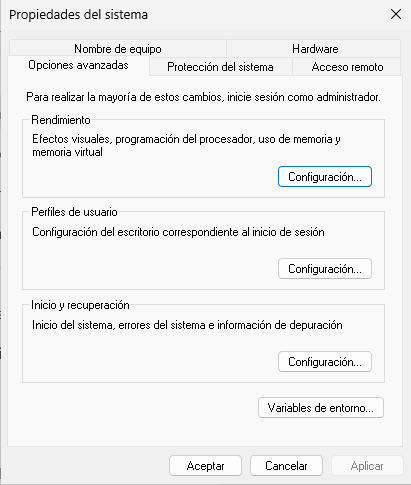
\includegraphics{sysdmcpl.png} \# Com definir o modificar variables
d'entorn

\subsection{Definir temporalment (durant la sessió CMD
actual):}\label{definir-temporalment-durant-la-sessiuxf3-cmd-actual}

\begin{Shaded}
\begin{Highlighting}[]
\BuiltInTok{set} \VariableTok{NOM}\NormalTok{=valor}
\end{Highlighting}
\end{Shaded}

Exemple:

\begin{Shaded}
\begin{Highlighting}[]
\BuiltInTok{set} \VariableTok{PROVA}\NormalTok{=Hola món}
\BuiltInTok{echo} \PreprocessorTok{\%}\VariableTok{PROVA}\PreprocessorTok{\%}
\end{Highlighting}
\end{Shaded}

\subsection{Definir permanentment (a través de l'entorn
gràfic):}\label{definir-permanentment-a-travuxe9s-de-lentorn-gruxe0fic}

\begin{enumerate}
\def\labelenumi{\arabic{enumi}.}
\tightlist
\item
  Escriu \texttt{SystemPropertiesAdvanced} en el CMD i prem Enter.
\item
  Fes clic a \textbf{Variables d'entorn}.
\item
  Afegeix, edita o esborra variables d'usuari o del sistema.
\end{enumerate}

\begin{quote}
No es poden modificar variables de sistema des del CMD sense usar eines
com PowerShell o \texttt{setx}.
\end{quote}

\begin{center}\rule{0.5\linewidth}{0.5pt}\end{center}

\section{Ús habitual de variables
d'entorn}\label{uxfas-habitual-de-variables-dentorn}

\begin{itemize}
\tightlist
\item
  En scripts \texttt{.bat} per fer referència a carpetes i usuaris:
\end{itemize}

\begin{Shaded}
\begin{Highlighting}[]
\BuiltInTok{copy}\NormalTok{ fitxer.txt }\PreprocessorTok{\%}\VariableTok{USERPROFILE}\PreprocessorTok{\%}\NormalTok{\textbackslash{}Documents\textbackslash{}}
\end{Highlighting}
\end{Shaded}

\begin{itemize}
\tightlist
\item
  Per controlar el comportament d'aplicacions i instal·ladors
\item
  Per configurar entorns de desenvolupament (per exemple,
  \texttt{JAVA\_HOME}, \texttt{PYTHONPATH})
\end{itemize}

\end{document}
